\documentclass[10pt,conference,onecolumn]{IEEEtran}

\usepackage[utf8]{inputenc}
\usepackage{hyperref}
\hypersetup{
  colorlinks, linkcolor=blue
}

\usepackage[a4paper, total={5.8in, 9in}]{geometry}
\usepackage{graphicx} % For figure environment
\usepackage{subfig}
\usepackage{gensymb}
\usepackage{siunitx}
\usepackage{caption, float}
\usepackage{booktabs}
\usepackage{siunitx}
\usepackage{array}
\usepackage{dirtytalk}
\usepackage{tikz}

\usetikzlibrary{positioning}

\begin{document}

\tikzset{%
  every neuron/.style={
    circle,
    draw,
    minimum size=0.5cm
  },
  neuron missing/.style={
    draw=none, 
    scale=3,
    text height=0.333cm,
    execute at begin node=\color{black}$\vdots$
  },
}

\title{Simulating a football game}

\author{
  Valentin Moullet\\
  \textit{Artificial Intelligence Laboratory (LIA), EPFL, Switzerland}
}

\maketitle

%%%%%%%%%%%%%%%%%%%%%%%%%%%%%%%%%%%%%%%%%%%%%%
\section{Introduction}
Sports have always been very important in our culture, especially football (or soccer for Americans). People have favorite teams, they root for them, make bets with friends about which team will win which games and so on. There is also a very big industry in football betting, in which there are bookmakers that set odds for games (saying, for example, if team A wins I will give you 1.5 times the amount you bet), and people bet on those odds trying to earn money. It is very obvious that both bookmakers and bettors would benefit a lot by being able to predict accurately the outcome of the games: the bookmakers by setting better odds that will give them less chance of going bankrupt, and the bettors by betting more accurately on games.

At the beginning, and still a bit today, predictions were done by experts following specific leagues and teams very closely, knowing a lot about football and being trusted by a lot of people. Then some people tried to apply statistical tools; this became quite popular around the 90s (even though the first statistical model was suggested by M. J. Moroney in 1956 \cite{facts_from_figures}). Then, more recently, with the available data all over the Internet, we logically saw the rise of machine learning trying to create models able to predict more accurately those results. All in all, trying to predict the outcome of a football game has been done for a long time and using a lot of different techniques.

Besides prediction, another important aspect is to understand how the game evolves over the time and to understand it better, keeping in mind its complexity and the different events that occur. This could be beneficial for teams who would like to improve their game, to understand how their team performs in different situations and to get an idea of what need to be changed in their strategy to improve.

What we are focusing on in this paper is more about the second aspect than the prediction of the results. We are interested in generating the sequence of events that will happen in a football game between two specific teams. Those events can be goals, shots, fouls, corners, etc... In other words, we want to model the distribution of the sequences of events that occur during a game. Being able to generate those with a good precision has nice side effects, such as predicting the outcome of a game. A more direct useful application of being able to generate such events is using it in games where you want to automatically generate games, such as football management simulation games (e.g. the Football Manager\footnote{See \url{http://www.footballmanager.com/} for more information about the game.} series). Indeed, in those games you act as the manager of a team, putting strategies in place for your team, and then letting the game being generated. Of course, players play a big role, but our work doesn't cover the impact of players; this is although something that could be done in the future with our work.

In order to generate a sequence of events in a football game, we're proposing the use of recurrent neural networks (RNNs). Indeed, RNNs can be trained for sequence generation by processing real data one step at a time and predicting what should be next. The predictions will be probabilistic, which means that we can generate events step by step from a trained network by sampling from the output distribution of the network and then feeding in the sample as input to the next step. Since we sample from a distribution, there will still be stochasticity and games will look different, even with the same teams playing. Of course, this means that the distribution at each step is conditional on the previous sampled events. It is known that, in principle, RNNs are not able to keep information about past inputs for very long \cite{Hochreiter01gradientflow}. This is a problem for us because we know that an event in football doesn't only depend on the few last events, but on the current state of the game and thus on almost all previous events (e.g. is the team losing or winning).

An architecture has been designed to better store and access information than standards RNNs, leading to having a way better memory. This architecture is called Long Short-Term Memory (LSTM) \cite{lstm}. It has already been shown to be the go-to strategy in different sequence processing tasks, such as speech and handwriting recognition, by producing very good results \cite{speech_recognition, NIPS2008/handwriting_recognition}. In this work, we want to show that it's possible to generate realistic sequences of events in football games with LSTM.

Section \ref{sec:related_work} presents some work related to the problem we're trying to solve. Section \ref{sec:problem_statement} states the exact problem we want to solve, and shows what data we have available to help us solve it. Section \ref{sec:simple_nn} introduces a simple neural network whose goal is only to predict the outcome of a game between two teams; some weights of this network will be used as features for teams in our RNN. Section \ref{sec:rnn} describes our main model built using the LSTM architecture and presents the different results we obtain with it. Section \ref{sec:discussion} contains some high-level discussions about the model, the results and their meaning. Finally, concluding remarks and directions for future work are given in Section \ref{sec:conclusion}.


%%%%%%%%%%%%%%%%%%%%%%%%%%%%%%%%%%%%%%%%%%%%%%%

\section{Related Work} \label{sec:related_work}
RNNs are quite used when working with sequences of events, when, for example, trying to learn phrases and words \cite{DBLP:journals/corr/ChoMGBSB14} or, more recently, generating sound from images \cite{rnn_sound}. Indeed, unlike simple multilayer perceptron, RNNs have an internal state, similar to some kind of memory. Sadly, in practice, this memory is very limited and forgets previous elements in sequences very quickly. This is where LSTM network comes in handy, each unit of this network is composed of a cell, an input gate, an output gate and a forget gate. The cell is responsible for the so-called memory, and the gates are there to regulate the flow of the network. Thanks to LSTM, RNNs are now better at problems needing a lot of memory, such as speak recognition \cite{speech_recognition} and handwriting recognition \cite{NIPS2008/handwriting_recognition} as said in the introduction.

In general, there has been quite some work done to try to predict the outcome of football games: home team wins, away team wins, or they make a draw.

In 2004, Goddard \& Asimakopoulos \cite{goddard} are using a probit regression model and 15 years of all kinds of data from the English Premier League (EPL) to predict the outcome of games and try to make money betting using the bookmakers' odds. They showed that they would have been able to generate a positive return of at least 4\% in the four most recent seasons by betting on well-known bookmakers. Their work shows that information such as which cities the games took place, the importance of the games (promotion, relegation), the teams' involvement in cup competition and other data not relative to past games also have some predictive quality, although in our work we don't use such precise information.

In 2013, Kumar \cite{ml_kumar} used different machine learning techniques in order to predict the outcome of football games. In his work, he showed that by using players' ratings from past games, then putting them together for all players in a team to build teams' ratings, he could predict correctly the outcome of around 53\% games with the best techniques such as Neural Networks and Support Vector Machine.

Maystre, Kristof, Gonzalez Ferrer \& Grossglauser \cite{Maystre:221151} also show how it is possible to measure a team's strength based on the players' contribution. They trained their model with games between clubs, but applied their method on Euro 2008, Euro 2012 and Euro 2016, which are only games between countries, to find out their predictions were really competitive with the ones made by the bookmakers, even though this conclusion seems to be quite rushed because the numbers of games in those tournaments are really low (31, 31 and 51 respectively). This still seems to show that the players play a very big role in how strong a team is. You can see some graphs about the strengths they give to the teams over time at \url{http://kickoff.ai/teams}. Trying to represent a team by a score, or by a multidimensional data point, clearly seems to help predicting the outcome of games. We will see how we want to do that in our case.

More recently, in 2017, Pettersson \& Nyquist \cite{rnn_players_prediction} used RNNs (with an LSTM architecture) to try to predict the final outcome of a football game as the game goes on (every 15 minutes more precisely), which of course makes the accuracy go up as the game goes on. They're using events happening to the different players during the game in order to predict the final outcome. Their accuracy at the start of every game is not very high (less than 45\% of the games predicted correctly), but goes up as the game goes on (i.e. more than 50\% at the half-time, 74\% at the 75th minute). The idea seems reasonable, but the way to compute the accuracy as the game goes on doesn't seem a good indicator of how well the events happening are helping the network. Indeed, it would have been better to compute the accuracy of only the second part of the game as the game goes on, which should result in slightly better accuracies as more events already happened.

We couldn't find any work directly related to generating sequences of events in a football game (or any other sport), but as said before, there has definitely been some work in sequence processing with an LSTM architecture in other fields, such as in speech recognition by Graves, Mohamed \& Hinton, 2007 \cite{speech_recognition}, where they broke the current record on the TIMIT\footnote{See \url{https://catalog.ldc.upenn.edu/ldc93s1} for more information.} phoneme recognition benchmark, in handwriting recognition by Graves \& Schmidhuber, 2009 \cite{NIPS2008/handwriting_recognition}, where they were able to beat all scores in an Arabic handwriting recognition (despite not knowing any words in Arabic). More recently, in 2014, Graves \cite{generate_events_lstm} showed that it was possible to generate complex sequences of events, such as texts (typed and handwritten), by predicting one data point at a time. The results are quite impressive and shows how powerful LSTM architectures are for generating those kind of sequences. This last paper is very interesting for our work, because, by abstracting it, what we want to do is quite similar: generating sequences of events one data point at a time based on the previous data points. For example, the paper explains how at each step, when generating a sequence, they predict the probabilities of the possible events, and then sample from those probabilities to get a concrete event, which they can use as input in the next step.

With this knowledge, we are quite confident in the fact that generating realistic sequences of events in a football game should be possible, and is something new in the field of predicting and understanding sports games.

\section{Problem statement} \label{sec:problem_statement}
Our goal is to create a model that is able to generate a realistic sequence of events in a football game between two teams, and that the generated events are close to what would happen in reality. The generated events should depend on the teams playing, their sides (playing home or away) and the previous events in the game (e.g. very likely to have a goal after a penalty).

\subsection{Data}
To achieve that, the first challenge is to find appropriate data. The data we used was taken from Kaggle, put online by Alin Secareanu\footnote{See \url{https://www.kaggle.com/secareanualin/football-events/data}.}. Most data were scraped from \url{http://www.bbc.com/}, \url{http://www.espn.com/} and \url{https://onefootball.com/}. It contains two important CSV files: ginf.csv and events.csv.

The first one contains a list of 9074 games from the best league of England, France, Spain, Italy and Germany, between the 2011/2012 season and the 2016/2017 season. Every game comes with the corresponding league, date, final score, the best odds given by any bookmaker referenced on \url{http://www.oddsportal.com/} and some other information.

The second one contains a list of events for almost each game present in the previous list. There is a total of 941009 events. An event contains the time (in minute) it happened in the game, which team was the actor of it, what is the event type (represented by a number), the player that was the the main actor of the event and some other information. Here is a list of the different event types with their percentage of appearance in the dataset:
\begin{itemize}
  \item Goals (2.5\%)
  \item Attempts/shots (21.8\%)
  \item Corners (9.7\%)
  \item Fouls (24.7\%)
  \item Yellow cards (4.2\%)
  \item Second yellow cards (0.01\%)
  \item Red cards (0.1\%)
  \item Substitutions (5.5\%)
  \item Free-kicks won (25.3\%)
  \item Offsides (4.6\%)
  \item Handballs (1.1\%)
  \item Penalties conceded (0.3\%)
\end{itemize}

We split all those games into a training set (70\% of the games) and a test set (30\% of the games). Note that the games were sorted by date, and thus the test set contains only games that happen after all the games in the training set, in order to be as real as possible.

\subsection{Statistics}\label{ssec:statistics}
It can be interesting to see when some events happen during the game. For example, does the number of goals diminishes or rises as the game goes on because of players getting more tired? Is there indeed more substitutions of players during the second half of the game, as one would indeed expect? This is interesting to see, and it will be interesting to check if our model is able to understand this. Figure \ref{fig:goals_distr} shows how the goals are distributed during the games, and Figure \ref{fig:substitutions_distr} shows the distribution of when the substitutions happen.

\begin{figure}[H]
\centering
\includegraphics[width=125mm]{images/goals_distr}
\caption{The distribution of all the goals in the dataset throughout the time of a game.}
\label{fig:goals_distr}
\end{figure}

\begin{figure}[H]
\centering
\includegraphics[width=125mm]{images/substitutions_distr}
\caption{The distribution of all the substitutions in the dataset throughout the time of a game.}
\label{fig:substitutions_distr}
\end{figure}

Note that we mostly have peaks during the 45th and the 90th minute because, for the 45th minute, all events happening in the additional time of the first half are referenced to be happening at the 45th minute, and the same for the 90th minute, except that some sources sometimes wrote down the events happening in the additional time with their real time.

As we can see, the number of goals slightly increases as a game goes on, which could be explained by the teams taking less risk at the beginning of a game, or maybe the freshness of the players arriving on the field later having a lot of impact, because we indeed see in the second figure that most substitutions happen during the second half of the game, and a lot of them during the half-time break.

Another interesting statistics we would want to see is how an event affects the possible next ones. In other words, it would be nice to see the different events and how likely it is to have each event happening after the previous one. We can compute that for each pair of event by counting the number of times it happens, and then dividing by the total number of events of the type of previous event. Then, in order not to depend on the total number of the next event (e.g. there are way more fouls than substitutions), we should divide by the general probability of this event happening (number of times it happened in the dataset divided by the total number of events in the dataset). We then obtain a number which says how much the previous event increases the fact of having the new event. It is important to do that separately for previous and next events happening to the same team and to different teams, since, for example, a team conceding a penalty would increase the chances of having a red card for the same team, but not for the other team. You can see the corresponding tables in a heatmap form in Figure \ref{fig:same_side_event_influence} and in Figure \ref{fig:other_side_event_influence} respectively. Keep in mind that, in reality, not only the direct previous event affects the next one.

\begin{figure}[H]
\centering
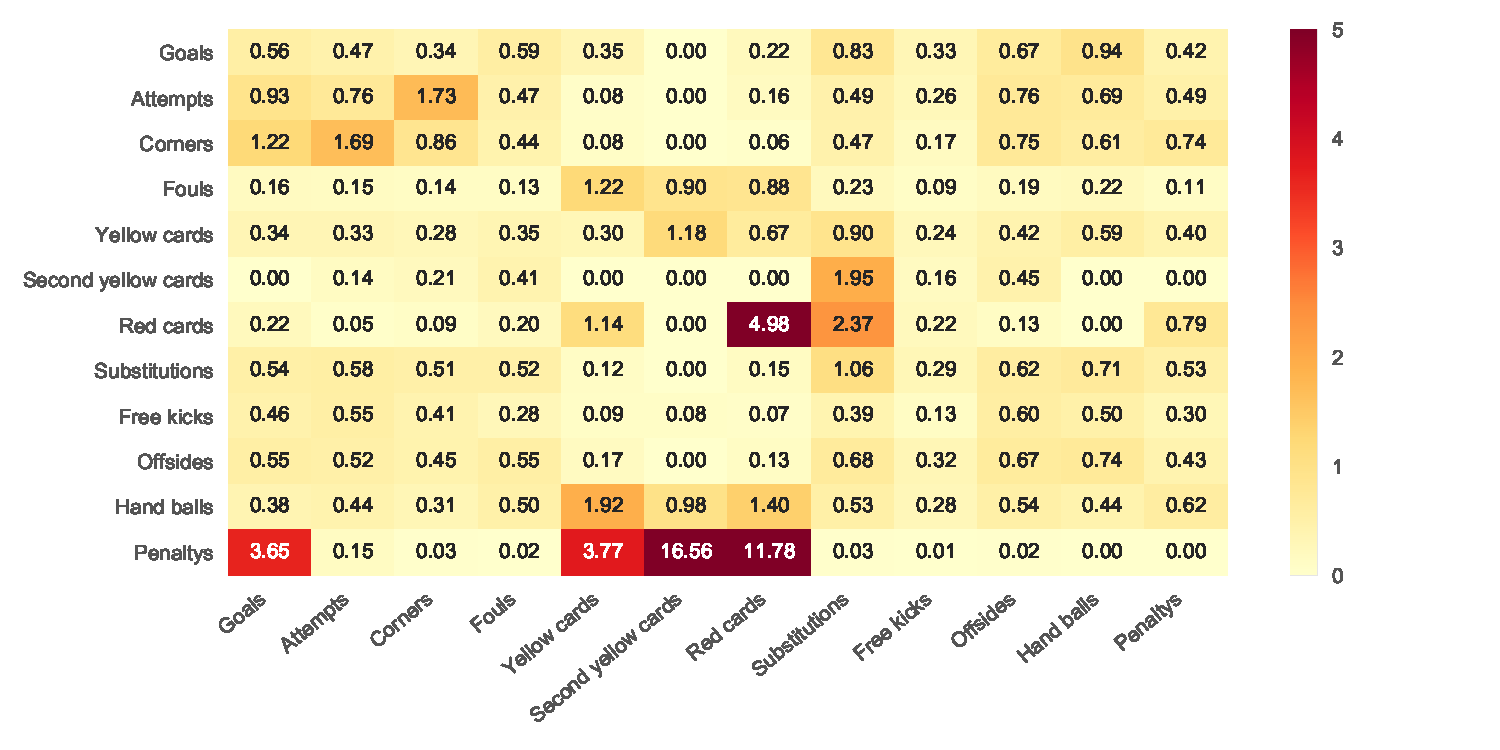
\includegraphics[width=125mm]{images/same_side_event_influence}
\caption{Heatmap showing how the previous event (y axis) increases the likelihood of having the next event (x axis) for the same team.}
\label{fig:same_side_event_influence}
\end{figure}

\begin{figure}[H]
\centering
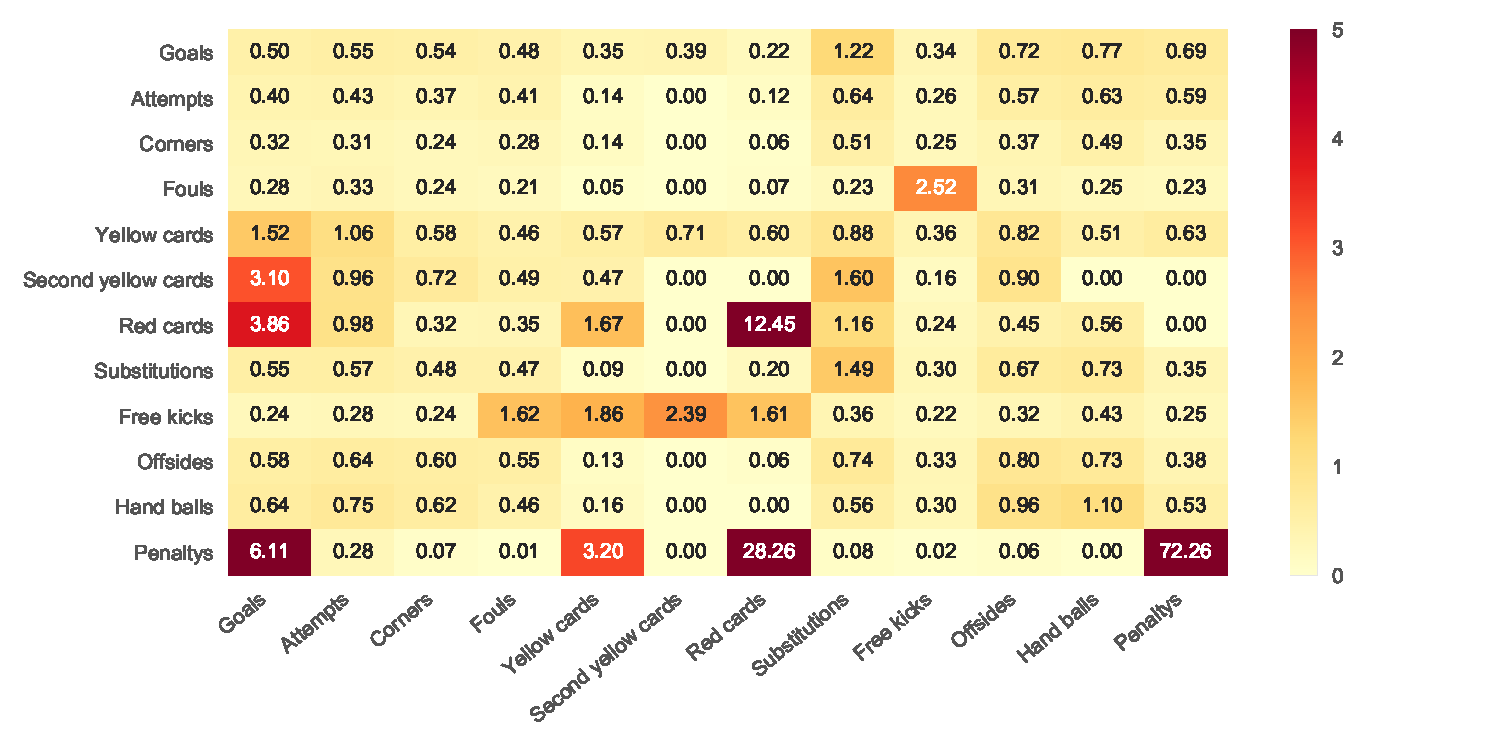
\includegraphics[width=125mm]{images/other_side_event_influence}
\caption{Heatmap showing how the previous event (y axis) increases the likelihood of having the next event (x axis) for the other team.}
\label{fig:other_side_event_influence}
\end{figure}

Those tables show us indeed what we could have been expecting, like having a team having an attempt increases its chances to get a corner, or a team conceding a foul will likely result in a free kick for the other team, but they also raise some questions about the data. Indeed, we can see that this is very likely to have a yellow card followed by a foul for the same team, but having a foul followed by a yellow card also seems likely. Also, a penalty for a team is likely followed by a goal for the other team, which seems weird. How this can be explained is that the sources that wrote the events didn't agree on the order of putting some events (first yellow card or foul?), and the meaning of some events (is it penalty won or conceded?). This could lead our model to confusion about some specific situations, and it will be interesting to see how it adapts, but otherwise, in general, we want to see if our model follows similar transition rules.

%%%%%%%%%%%%%%%%%%%%%%%%%%%%%%%%%%%%%%%%%%%%%%%%
\section{Simple neural network for predicting winner} \label{sec:simple_nn}
As said before, our main goal is to accurately predict events that will happen in a game with two teams facing each other. One thing that would help us greatly to know what kind of events will happen in a game between two teams would be to have some kind of features for those teams, helping the model to understand what type of teams are playing each other.

By creating a neural network trying to predict the outcome of a game between two teams, we think we can extract useful information about those teams. Thus, the goal of this neural network is to predict, given two teams, one playing home and the other away, what are the probabilities of the three possible outcomes: home win, away win and draw?

\subsection{Model}\label{ssec:simple_model}
The network is taking as input two one-hot vectors of the length of the number of teams in the league, each representing a team (one vector for the home team, one vector for the away team), and outputting probabilities of the outcome of the games (home win, away win, draw). The network also contains two hidden layers which should be useful for having some kind of latent features for the teams. You can see its architecture in Figure \ref{fig:simple_nn}.

\begin{figure}[H]
\centering
\includegraphics[width=85mm]{images/simple_nn}
\caption{Neural network for predicting winner of game. Note: the weights between the input layer and the first hidden layer are the same for the home team and the away team (highlighted in red).}
\label{fig:simple_nn}
\end{figure}

Note that the weights between the input layer and the first hidden layer are the same for the home team and the away team (highlighted in red).

What we expect from this network is that the final weights between the input layer and the first hidden layer will correspond to some latent features for each team. Also, each time we predict a game between two teams, the values contained in the second hidden layer should correspond to some latent features that the network learned when team A plays home and team B plays away. Indeed, we expect the network to automatically learn some important features about the teams to help for the prediction task, features which could be interpreted as how strong is the team in attack, in defense, when playing home or away, etc... Those features will come in handy later when predicting and generating events, in order to have more information about the teams playing against each other. We will convince us that those features are meaningful in Section \ref{ssec:teams_features}.

In order to find the best hyperparameters for our network, we used grid-search. You can see the values that were searched and the best values overall in Appendix \ref{appendix:hyperparams_simple_nn}. Also, for the activation function, we used the rectified linear unit (ReLU \cite{relu}) due to its famous efficiency, and we trained our model using Adam \cite{DBLP:journals/corr/KingmaB14} as optimization algorithm. Since we output probabilities, we use the cross entropy loss as the loss for our model. Note that it would have been even better to also try different optimization functions as well as multiple activation functions, but due to time constraint we decided to go with those, which are known to be good.

\subsection{Evaluation}

\subsubsection{Accuracy estimation} \label{ssec:accuracy}
Even though this isn't our final model and our focus is not on how accurately we can predict a game's outcome, it is still interesting to see how our simple model is doing against the bookmakers. But also, it will give more credibility to the latent features we described earlier if our model gives good prediction.

Bookmakers have to give odds, so they want to know as good as possible the probabilities of the three possible outcomes in order to give the best odds and take less risk. Indeed, bookmakers give odds in the form of a number strictly bigger than 1, which represents how many times you'll get back the amount you bet if you bet correctly (e.g. if the odds for draw are of 2, you'll get 2 times the amount bet if the game indeed ends in a draw). From the odds, you can get a good approximation of what probabilities bookmakers would give to each outcome: you just have to take $\frac{1}{odds}$. Ideally, you want the following: 
$$\frac{1}{odds\_home\_win} + \frac{1}{odds\_away\_win} + \frac{1}{odds\_draw} = 1$$
But bookmakers generally make it such that this sum becomes bigger than 1 in order to have a safe margin. Then, to get a better estimation of the probabilities, we can divide the current probability by the sum of the probabilities. We then have:
$$P(outcome=home\_win) = \frac{1}{odds\_home\_win} \cdot \frac{1}{\sum{\frac{1}{odds}}}$$
$$P(outcome=away\_win) = \frac{1}{odds\_away\_win} \cdot \frac{1}{\sum{\frac{1}{odds}}}$$
$$P(outcome=draw) = \frac{1}{odds\_draw} \cdot \frac{1}{\sum{\frac{1}{odds}}}$$
Now that we know that both ourselves and the bookmakers are actually assigning probabilities to each possible outcome, we want to find a way to compare both accuracies. In other papers, people are often computing their accuracy by counting how many games they predict correctly out of all the games. This is not really what we want, because our goal (and the bookmakers' one) is to give good probabilities on the possible outcomes. So our way to compute the accuracy is the following: the total accuracy is the mean of all games' accuracy, and a game's accuracy is the probability that was given to the actual outcome. For example, if you predicted $0.5$ for a home win, $0.3$ for a draw and $0.2$ for an away win, and that the outcome is a draw, this game's accuracy is $0.3$. This means that a very naive model would get an accuracy of $0.\overline{3}$ by always predicting $0.\overline{3}$ for each possible outcome.

You can see in Figure \ref{fig:all_leagues_accuracy} the total accuracy (average accuracy over all the games in the test set) of the bookmakers and our simple model for the five different leagues.

\begin{figure}[H]
\centering
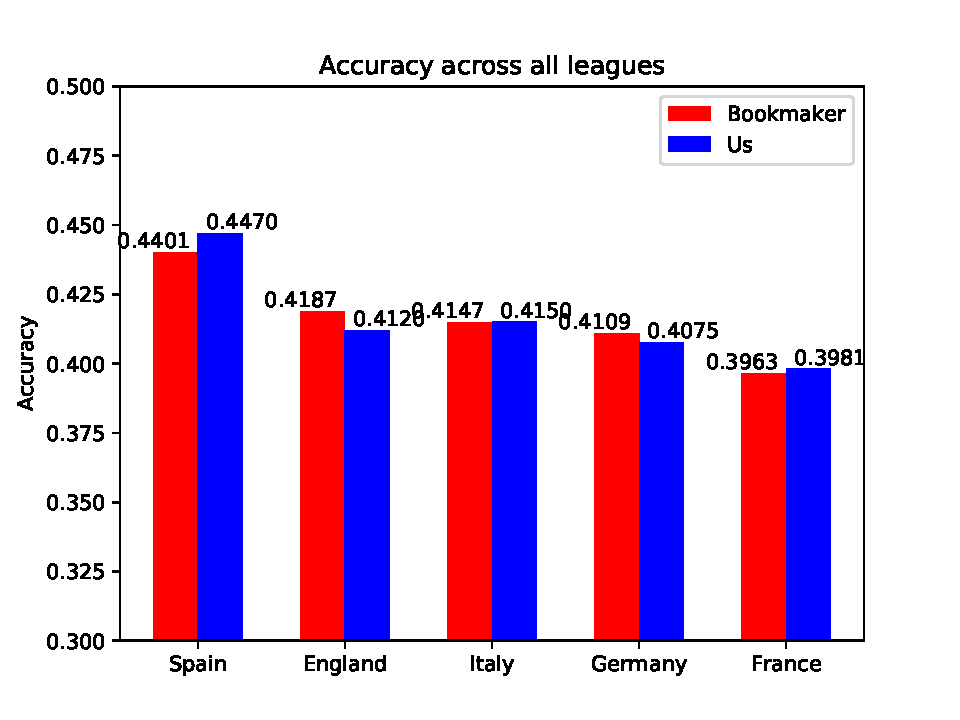
\includegraphics[width=85mm]{images/all_leagues_accuracy}
\caption{Bookmaker's and our average accuracy across all leagues over all games in the test set.}
\label{fig:all_leagues_accuracy}
\end{figure}

As we can see, the bookmakers are a bit better than us, but this is very close and quite impressive that with such a simple model taking only a short history of the teams' results into account we could almost get to their level.
\newline

\subsubsection{Teams latent features}\label{ssec:teams_features}
We are now interested to see if the latent features learned by the network (as discussed in Section \ref{ssec:simple_model}) have some interesting meanings. Since the best size of the first hidden layer of our model is 20 (as discussed in Appendix \ref{appendix:hyperparams_simple_nn}), each team have 20 features. We would like to display the different teams on a plot to see if we can identify clusters or outliers that would represent similar teams or very strong/weak teams. Since it's not possible to have a meaningful display in 20 dimensions, we can use dimensionality reduction on the teams latent features, keep only 2 dimensions, and then display the teams on a plot. We expect to see teams with a similar level clustered together, and the very strong teams being outliers. To help knowing how good a team is considered, the radius of the circles representing the teams has been increased for the strong teams: the bigger the radius is, the stronger the team is\footnote{We computed the strength of the teams using the website \url{http://footballdatabase.com/}.}. We can see what this gives for the English league and for the Spanish league, in Figure \ref{fig:england_weights} and Figure \ref{fig:spain_weights} respectively, with the use of a technique for performing a nonlinear form of Principal Component Analysis on the teams latent features, developed in 1999 by Schölkopf, Smola \& Müller, called Kernel PCA \cite{kernel_pca}.

\begin{figure}[H]
\centering
\includegraphics[width=100mm]{images/england_weights_size}
\caption{Representation of the latent features of teams in the English league after Kernel PCA \cite{kernel_pca}. The bigger the radius is, the stronger the team is (strength taken from \url{http://footballdatabase.com/}).}
\label{fig:england_weights}
\end{figure}

\begin{figure}[H]
\centering
\includegraphics[width=100mm]{images/spain_weights_size}
\caption{Representation of the latent features of teams in the Spanish league after Kernel PCA \cite{kernel_pca}. The bigger the radius is, the stronger the team is (strength taken from \url{http://footballdatabase.com/}).}
\label{fig:spain_weights}
\end{figure}

We clearly see big outliers on the left of the plots, such as Manchester City, Manchester United and Chelsea in the English league, as well as Barcelona, Real Madrid and Athletico Madrid in the Spanish league. In the Spanish league, we then see a big cluster containing the other teams, with Valencia and Sevilla standing out a little bit. This shows that the league has clear leaders, and could explain why it seems easier to predict than other leagues (see Figure \ref{fig:all_leagues_accuracy}). For the English league, we also see some other good teams, such as Arsenal, Tottenham and Liverpool being among what we could call the cluster of good teams. It is quite obvious that going from left to right, more or less, the level of the teams seems to decrease, with a cluster of middling teams near the middle.

The way the teams are displayed on the plots shows that the latent features (as discussed in Section \ref{ssec:simple_model}) the model was able to find and assign to the teams are somewhat important and relative to the strengths of those teams; this gives them some credibility.

%%%%%%%%%%%%%%%%%%%%%%%%%%%%%%%%%%%%%%%%%%%%%%%%%

\section{Recurrent neural network for predicting events} \label{sec:rnn}
Now that we have teams features, we want to create a model that can generate a realistic sequence of events for a game between two teams. So based on which teams are playing and their latent features derived from the previous network, we want to have the most realistic sequence of events for this game.

Only generating a sequence of events wouldn't make much sense without knowing at what time those events are happening. For each event, we want to know the event type (e.g. corner for home team) and also at what minute it happened in the game. Keep in mind that football games are 90 minutes long.

\subsection{Model}
Our RNN is composed of LSTM units for predicting each step of the sequence for a game. This means that at each step, we want to predict two things: the type of event and the time it happened. We also want to know which team was the actor of the event. One way would have been to also separately predict the actor of the event, but by doing that we make it such that this probability is not affected by the type of event, which is wrong; for example, a goal shouldn't have the same probability to be for one team or the other. Thus, we decided to represent the types of events as being the actor and the event together. For predicting the minute of the event, it wouldn't make sense and would be too hard to predict the exact minute between 1 and 90 because we predict the events one after the other, in the order they happen in the game. One simpler way is to output, for each event, the probability that it happens during the same minute than the previous event or not. With that, we can have multiple events during the same minute, and also only a single one in one minute. The only thing we still cannot do, and that happens in football games, is to have a minute without any event. What we did to make it possible is adding another type of event representing this: a "no-event" type.

We now know what should be the output at each step exactly: the probability of the event type with the actor, and the probability of the event happening in the same minute than the previous one. For the input, what we want to have is the previous event (event type and actor, as well as the time information), represented as two one-hot vectors. Then, the hidden state of the network should be carrying on the current state of the game. Figure \ref{fig:lstm_unit} shows this in a picture.

\begin{figure}[H]
\centering
\includegraphics[width=85mm]{images/lstm_unit}
\caption{Picture of how a step in our LSTM architecture would look like with the previous event and time information as input.}
\label{fig:lstm_unit}
\end{figure}

The only thing we're missing is some information about the teams. Indeed, as we discussed in Section \ref{sec:simple_nn}, having some information about the teams that are playing when generating the sequence of events will help our network a lot. For example, if a really good team plays against a weak one, the network should be able to generally predict more attempts, corners or goals to the strong team.

Initially, we didn't take that into account at all and were just generating games between two teams with the input of each step being the previous event. It was generating games, but the events were totally independent of the teams playing, which of course was making the predicted results look really bad.

To avoid that and make the predicted events also dependent on the teams playing, the network should be aware of those teams in some way. So we initiated the hidden state of our network with the values found in the second hidden layer of our previous model (Figure \ref{fig:simple_nn}) when predicting the outcome of a game between the same teams (playing on the same sides) for which we are currently predicting the events. This way, our network should know from the beginning what kind of teams are playing. Practically, this didn't really work out, because the network seemed to forget about this, probably because other information were taking over in the hidden state. To parry that, we decided to put those latent features about the teams as well in the input. We thus concatenate the latent features with the information about the previous event, to create our input at each step.

When training our network, the input of each step will be the teams' features concatenated to the two one-hot vectors representing the actual previous event (except for the first step, whose input event will be a special "start of the game" event). This means that at each step, the network will try to predict what should be the next event. Note that it is only receiving information about the target game (i.e. real game) while training, and not using anything previously predicted. Also, note that only a fourth of the training set was used because the network was struggling with this much data. It seems that the model was overfitting very quickly without having time to pass by a state where it was making meaningful relationships. Figure \ref{fig:lstm_network} shows the network in more details.

\begin{figure}[H]
\centering
\includegraphics[width=125mm]{images/lstm_network}
\caption{Representation of our LSTM network when taking the teams latent features into account.}
\label{fig:lstm_network}
\end{figure}

For the testing part though (and also when generating sequences between two teams), the input will always be the teams' latent features concatenated with the event and time information sampled from the probabilities given by the output of the previous step. Note that when generating a game, the only way we have to know when to stop is to look at the current time, and stop after the 90th minute. Figure \ref{fig:rnn_test_network} highlights the discussed architecture.

\begin{figure}[H]
\centering
\includegraphics[width=100mm]{images/rnn_test_network}
\caption{Representation of our LSTM network when taking the teams latent features into account.}
\label{fig:rnn_test_network}
\end{figure}

When training our network, a simple way to compute the loss for each step would be to do the average of the cross-entropy loss between both the event type and time predicted probabilities and their target: the next event in the real game. This is what we did first, but the problem was that the network was easily entering in a special state of "looping". More precisely, the network was learning that after a foul by a team, there was a really big probability of having a free-kick for the other team in the same minute if there wasn't already a free-kick for the same team beforehand, but the network was also learning that after a free-kick for a team, there was a big probability to have a foul by the other team, in the same minute, if there wasn't already a foul for the same team right before. Now, if we are unlucky and that the network generates two fouls in a row, it knows that it should generate a free-kick at the same minute for the other team with high probability, but one is not enough because there was two fouls, so the network thinks it has to generate another free-kick in the same minute, and when it does that, it tries to generate a foul because a free-kick just happened, and we enter some kind of loop like this where we have a lot of fouls and free-kicks (mixed with some other events such as yellow cards) happening at the same minute. We think this is due to the fact that the sources from where we get the data didn't have a strict rule of putting the foul or the free-kick first, which made the network learn that both ways were extremely probable.

In order to counter this, we found two possibilities. The first one was to detect when this loop was happening (for example by checking if we already had 10 events at the same minute), and start again the generation of the game if we detect it, but this seemed too "manual". The second one was to add another loss for forcing the network to not generate too many events in the same minute in a row. To do that, we computed the ratio of events happening in the same minute than the previous event in the games in the training set (which is around 35\%), created a Beta distribution\footnote{See \url{https://en.wikipedia.org/wiki/Beta_distribution} for more precision about this distribution.} centered on 35\% by tweaking its $\alpha$ and $\beta$, and for each step, computed the logarithm of the probability density function of the Beta distribution evaluated at the value (probability) given by the network for having the next event at the same minute than the previous one, and then took its negative to have a decreasing loss as the network is getting better. In other words, we are regularizing the events happening at the same minute in order to avoid entering in those loops.

What remains to know is how to put those losses together. We have one cross-entropy loss coming from the events, one cross-entropy loss coming from the time information and one loss coming from the repetition of consecutive events at the same minute. What we did to put those losses together was to assign different weights to each of them and sum them up. In addition to those weights, the network contains multiple hyperparameters that could be tweaked in order to find the best network. By lack of time (the training of the network takes a long time), we didn't use any exhaustive grid-search, but manually changed some hyperparameters to have a good enough result. You can find more information about the hyperparameters in Appendix \ref{appendix:hyperparams_rnn}. The optimization algorithm that we used was again Adam.

\subsection{Evaluation}
\subsubsection{Predicting winner}
As explained in the introduction, generating realistic sequences of events for football games has the side effect of being able to predict the outcome of games. Although this is not the final goal, it would be nice to see how accurate those predictions are, compared to the bookmakers' ones and also the ones made when using our previous network described in Section \ref{sec:simple_nn}; the accuracy is computed using the same technique presented in Section \ref{ssec:accuracy}. Having a good accuracy would show that the events being generating (or more precisely the goals) are not completely random and correspond to the teams. Figure \ref{fig:rnn_accuracy} shows how the accuracy of our network compares for the first 40 epochs with the (already known) bookmakers' accuracy and the one of the previous network presented in Section \ref{sec:simple_nn}.

\begin{figure}[H]
\centering
\includegraphics[width=85mm]{images/rnn_accuracy}
\caption{Accuracy over epochs of our RNN about predicting the outcome of games in the test set, with the two already computed accuracies: the bookmakers' one and the one from our model described in Section \ref{sec:simple_nn}.}
\label{fig:rnn_accuracy}
\end{figure}

Remember that, as discussed in Section \ref{ssec:accuracy}, the accuracy we are using here is not computed the same way most of the papers compute it (e.g. 53\% by Kumar \cite{ml_kumar}): we are not interested in knowing for how many games we can predict the outcome correctly, but we want to give the most precise probabilities to each possible outcomes. In the end, our accuracy is closer to a cross-entropy loss, but with numbers that a person can relate to, at least a bit more.

We see that our network cannot reach the accuracies that the bookmakers, or even our previous network, can achieve, but is not that far. Note that even though on this graph, which was made during the training of the model, we only reach an accuracy of 40.3\%, this is a bit volatile because we only generate 10 times per game in order to see what are the probabilities of the outcomes for this game. For example, we were able to reach more than 41\% of accuracy with a similar model, but not during the training phase. The order of magnitude is still meaningful.

It is important to see that the model seems to learn how to predict the outcome of games over time, even though this is not what it was trained for. This shows that learning how to generate events realistically based on the teams has the side-effect of producing better final outcome predictions. Also, reaching such an accuracy with this model on the outcome gives us confidence for the generation of the other events.
\newline

\subsubsection{Predicting types of events}
A better way to see if our network learned anything related to the events is to observe if we generate a realistic number of goals, shots, corners, etc... For example, if we generate 100 times a certain game, we can look how many goals, shots, ... we generated each time, and then build a normalized distribution with it. For example, if there are 8 corners for the home team in a game, and that in 44\% of the time we generated 8 corners for the home team for this game, then the events distribution accuracy for the event type "corner home" for this game will be 44\%.

Now we want to compare our accuracy with baselines. A good baseline would be to take the normalized distribution of all the games in the training set for each event type. Indeed, it makes sense that games follow the same distribution in average, and if our network learned anything about the events and their relations with the different teams, we should have a better accuracy than this global one. Another good baseline would be to have different distributions for each team, where each distribution would be created out of the specific events done by the corresponding team. This second baseline is now also taking into account how a team plays and the events they generally have in their game; if our network was able to learn how playing home or away, or against what type of teams, affects the events happening in a game, it should also have a better accuracy than this second baseline. An example of those distributions and how we compare them for the number of shots made by TSG Hoffenheim in a specific game between TSG Hoffenheim and SC Freiburg is shown in Figure \ref{fig:example_distribution_shots}.

\begin{figure}[H]
\centering
\includegraphics[width=85mm]{images/example_distribution_shots}
\caption{Comparison of three different distributions on the number of events (here number of shots) in one game and how we score each of them based on the real number. This specific game is TSG Hoffenheim against SC Freiburg, and we're looking at the number of shots made by TSG Hoffenheim. First distribution is the one from the number of shots across all games, the second one is the one from the number of shots by TSG Hoffenheim across all games, and the third one is the distribution induced by the number of shots across 50 simulations of this game generated by our model. The actual number of shots by TSG Hoffenheim in this game is shown in red (i.e. 12 for this game).}
\label{fig:example_distribution_shots}
\end{figure}

If, for each type of event, we take the average of the accuracy over all games in the training set, we can then compare the overall accuracy for our three strategies: global distribution from the training set, team-specific distribution, and the distribution built from our solution when sampling multiple times each game. This comparison can be seen in Figure \ref{fig:events_accuracies} for key event types.

\begin{figure}[H]
\centering
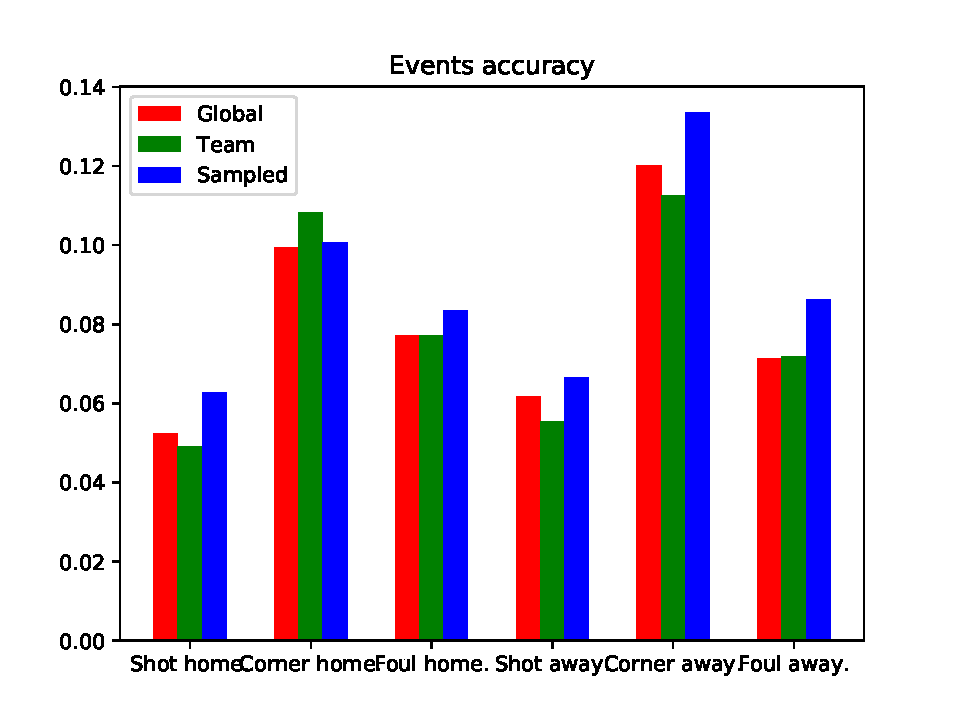
\includegraphics[width=125mm]{images/events_accuracies}
\caption{The events accuracies (correctly predicting the number of specific events happening in a game between two specific teams) for the most important events. Comparison between the global distribution of all games, the global distribution of the corresponding teams, and the distribution induced by generating multiple games with our model (called "sampling" here).}
\label{fig:events_accuracies}
\end{figure}

As we can see, the distribution accuracy of our network is in general better than the other ones. This gives us confidence that our network learned useful relationships between the teams, which side they're playing on and the events happening. We are now pretty sure that the events generated in a particular game should be relevant to the teams playing.

In order to say if our network generates realistic sequences of events, it remains to see how the different events influence each other, for example how does a corner for the home team influence the next event(s) being generated. We will address this later in Section \ref{ssec:qualitative}.
\newline

\subsubsection{Predicting parts of a game}
When making this model, we were thinking that one application would be to feed the network with the first half of the game, and let the network generate the rest of the game, and by comparing the generated outcome with the true outcome of the second half, it would be better than by giving nothing and only predict the second half. It turns out that it doesn't really change anything, we get approximately the same accuracies for both: around 37\%.

As you may notice, this accuracy is quite lower than the accuracy of predicting the outcome of the whole game with our model (around 41\%). We asked ourselves if it was because the second half was generally harder to predict than the first half of the game, so we tried to generate only the first half of the game and compute the accuracy. We were at first surprised to find out a similar accuracy (37\%) for predicting the outcome of the first half only.

One interpretation we can make from those results is that since our model has been trained to generate full games, it sees the game as a whole and does not focus on part of the games. For example, it knows it has time to "correct" unlucky mistakes (e.g. goals for the weak team) generated at the beginning of the game, so it might be bad during the first half, and then better during the second half. When being given the first half, it might realize that the strong team is already winning, and then not predict any goals for them in the second half, which could make the prediction for the second half wrong, but correct for the entire game. For our model, predicting the outcome of only a part of a game seems hard.

Additionally, we were wondering if it was hard for other models to predict the second half of a football game, or especially for our RNN implementation, so we designed a very simple neural network taking as input the current (first half) outcome and the teams latent features, and outputting the probabilities of the three possible outcomes of the second half of the game only, as you can see in Figure \ref{fig:half_nn}. You can also find more info about this network and its hyperparameters in Appendix \ref{appendix:half_nn}. We noticed that the network couldn't achieve really better than our previous one, only getting an accuracy of approximately 38\%, which is still worst than predicting the outcome of the whole game for any of our model. Keep in mind that the teams latent features were created out of full-time results of the corresponding teams. Thus, the reason why it seems hard to predict the second half (or the first half) only might be because the result of teams in a single half less corresponds to their strength in a full game.

\begin{figure}[H]
\centering
\includegraphics[width=85mm]{images/half_nn}
\caption{Simple Neural Network that takes the outcome of the first half of a game and the teams latent features in order to output the probabilities of the three possible outcomes of only the second half of the game.}
\label{fig:half_nn}
\end{figure}

\subsubsection{Qualitative analysis} \label{ssec:qualitative}
It now remains to see if the events are generated in an order that is realistic, meaning that, for example, a goal for the home team is highly probable after a penalty for them, or after a series of events near the other goalkeeper (corners, shots, ...). We couldn't find a good way to quantify this, so instead we are going to show some examples of how our model sees the probabilities of generating the events depending on the previous events. We will focus on a game between Real Madrid (home team), which is a strong team, and Elche (away team), which is a weaker team. You can see the probabilities of all the events at the very beginning of the game in Figure \ref{fig:test_0}. Note that the current minute of the game is written between squared brackets in the title of the figures.

\begin{figure}[H]
\centering
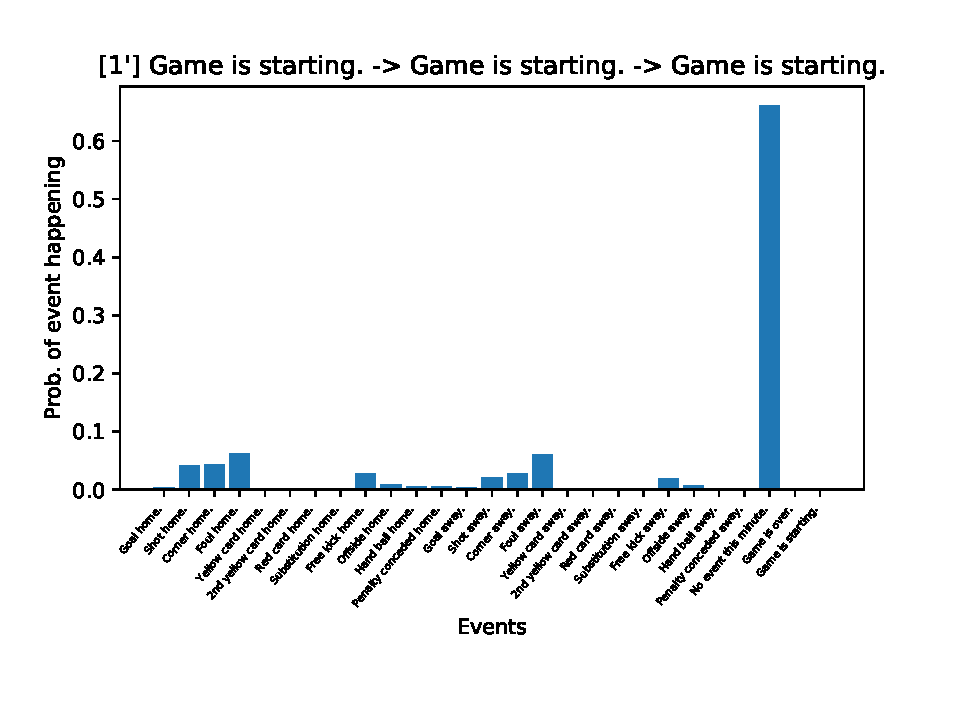
\includegraphics[width=125mm]{images/test_0}
\caption{Probabilities of all the different events at the very beginning of the game between Real Madrid (home team) and Elche (away team).}
\label{fig:test_0}
\end{figure}

We see that there is a high probability of having no event happening in the first minute, otherwise the rest seem to be pretty similar for both teams. Now, the network sampled a corner for the home team using those probabilities, and thus the probabilities of the events change drastically as you can see in Figure \ref{fig:test_1}.

\begin{figure}[H]
\centering
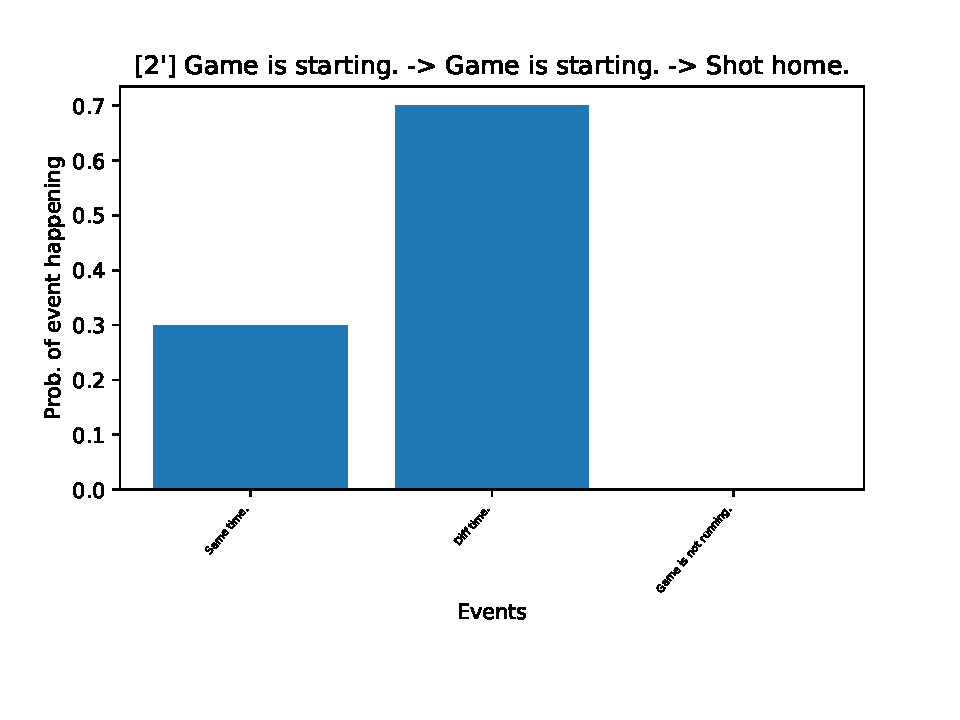
\includegraphics[width=125mm]{images/test_1}
\caption{Probabilities of all the different events after a corner for Real Madrid has been generated in the game between Real Madrid (home team) and Elche (away team).}
\label{fig:test_1}
\end{figure}

Indeed, we can see that all the events involving the home team as being the attacker increased a lot. This shows that the network recognizes the fact that the home team should be in this position when there is a corner for them.

Later on in the game, a penalty was generated for the home team. Figure \ref{fig:test_67} shows the probabilities that follows it.

\begin{figure}[H]
\centering
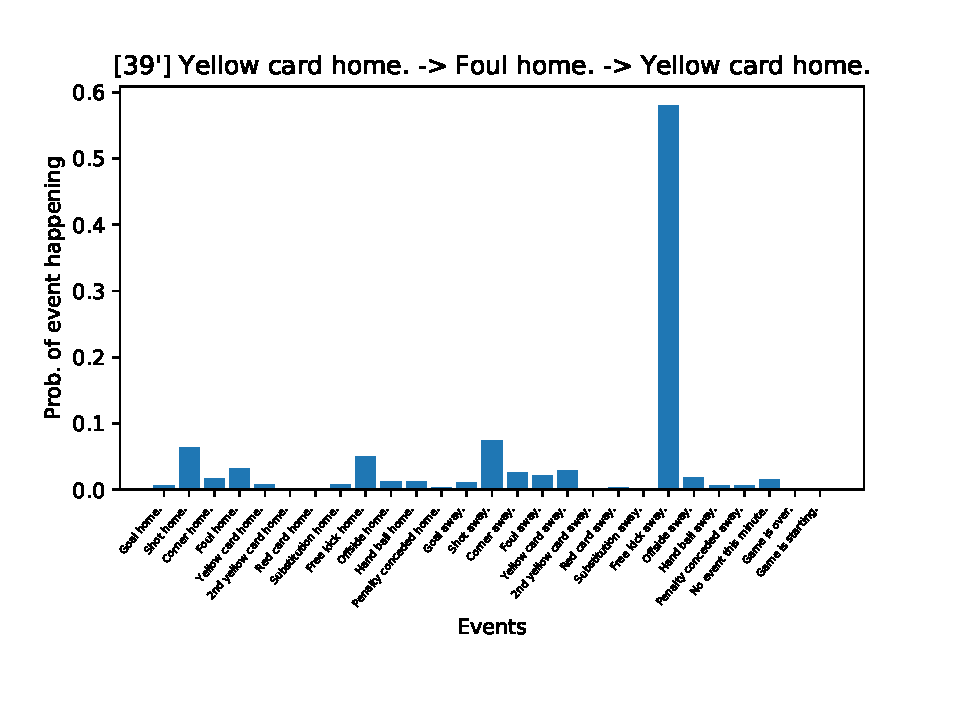
\includegraphics[width=125mm]{images/test_67}
\caption{Probabilities of all the different events after a penalty for Real Madrid has been generated in the game between Real Madrid (home team) and Elche (away team). You can see the three previous events in the title of the graph.}
\label{fig:test_67}
\end{figure}

As we can see, the probabilities of having a goal for the home team have increased by quite a lot compared to the previous ones, but not as much as we could have expected. This is due to the fact that the probabilities of having a yellow card for the away team is also huge after a penalty has been conceded by them (red card is also much higher than normal), and if the model would have sampled a yellow card or red card for the away team, it would then have increased much more the probabilities for the home team to have a goal. Sadly, this didn't happen in this game and the model directly sampled a goal for the home team.

A last example of later in the game is shown in Figure \ref{fig:test_126}, where the away team is in an offensive action: the previous events were a free-kick and a shot for them.

\begin{figure}[H]
\centering
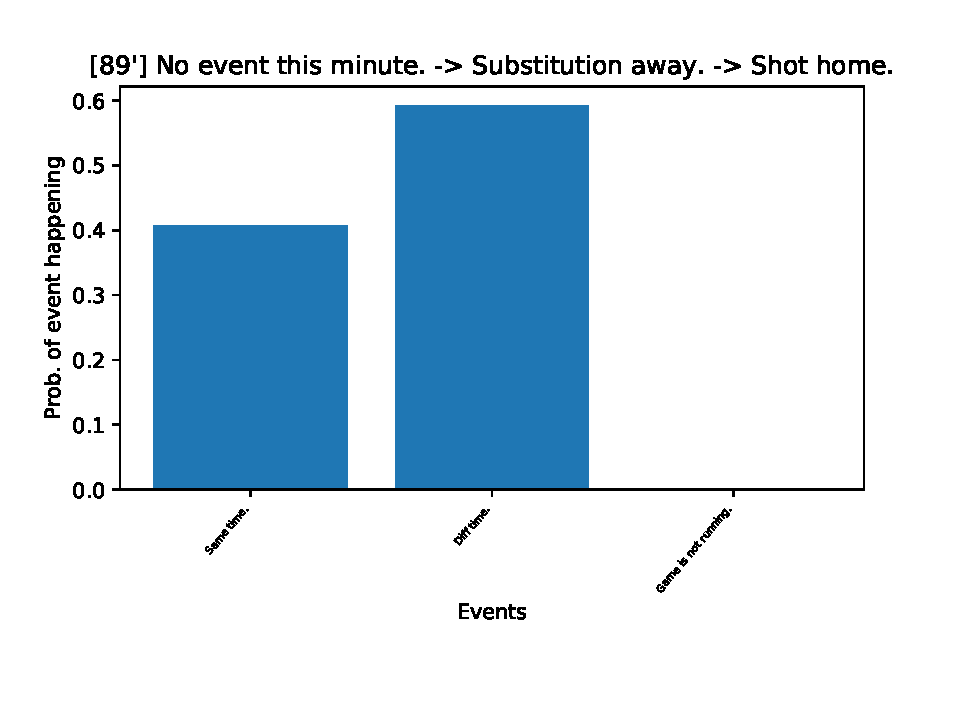
\includegraphics[width=125mm]{images/test_126}
\caption{Probabilities of all the different events during an offensive action from Elche at the end of the game between Real Madrid (home team) and Elche (away team). You can see the three previous events in the title of the graph.}
\label{fig:test_126}
\end{figure}

This last figure is interesting in order to see that when the weak (and away) team is having an offensive action, the probabilities of events involving them as the attackers do not extremely differ than the ones were the home team is the attacker (at least not as much as we can see in Figure \ref{fig:test_1}). This is due to the fact that the network knows that the home team generally has an advantage over the away team, and also that, in this case, the home team is clearly stronger than the away team.

Another interesting thing to note in this last figure is how the probabilities of having a substitution are high, especially compared to the first figures. This shows that the model keeps track of the time and know that at the end there are higher chances of seeing a substitution.

More figures and techniques about evaluating how good the previous events and the current state of the game can be found in Appendix \ref{appendix:qualitative}.

\section{Discussion} \label{sec:discussion}
In general, we see that the model we created is able to generate realistic sequences of events that seem to be better indicators of the kind of events that are going to happen in a game between two teams than just taking what happens normally in a football game or in games played by the corresponding teams. The model seems to understand the relationships between events, such as a goal for the home team is more probable after a corner for this team than after an offside from the other team for example.

We realized that the network can enter an unwanted state of "looping" because of the nature of the data we use. We believe there should be other ways of avoiding this issue than adding an additional loss as we did. One way would have been to remove all fouls from the dataset, since they really seem unnecessary since we already have the free-kicks and penalties; sadly, we thought about it too late.

We've learned that predicting the outcome of only a part of a game (such as the second half) was not only more difficult for our model (which is not focused on that), but also for a more simple model whose focus is only on predicting the second half outcome correctly knowing the first half outcome.

As said in the introduction, the goal for most people working in this area is to predict the outcome of the games. We've shown that our model is not as good as the bookmakers or the neural network we presented in Section \ref{sec:simple_nn}, but we clearly are not far. This gives us even more confidence in the events our model is generating because it wasn't even trained for predicting the correct outcome, this is only a side-effect of generating the events in a realistic way.

\section{Conclusion and further work} \label{sec:conclusion}
In conclusion, we showed that by generating sequences of events in football games using an RNN with an LSTM architecture, helped by teams features generated from their previous results, it was possible to make fairly good predictions on the outcome of games (home win, draw, away win), slightly under the bookmakers' ones. More importantly, we showed that our network was able to realistically generate those sequences of events depending on which teams were playing and was predicting, for almost each type of event, a more accurate number of events in games than baselines such as using the distribution of those events across all games or for specific teams. We believe to be the first ones to publicly focus on realistically generating such sequences of events in football games, and even in any sport; we think this work can be useful for sport management simulation games and also for real teams and coaches in order to understand, with a different view, how a game might evolve after certain key actions.

We strongly believe that more work can be done using this work as a starting point, or even as an inspiration. We clearly think that more time spent on this work would make it better; for example, we didn't have enough time to try out more combinations of hyperparameters or cleaning the model (i.e. removing the useless fouls), which is something that might improve the model. Also, we didn't take into account the players in order to create the teams latent features, and those features are static throughout all seasons and do not evolve with time, but they should if we want to be more accurate. It could also be nice to be able to not only say which team is the actor of an event, but the specific player(s). This could help the network to adapt when, for example, a strong player receives a red card, or even a yellow card, or when an important substitution occurs. We also think this technique could be applicable to multiple other sports, like handball or basketball.

\bibliographystyle{abbrv}
\bibliography{./literature}

\begin{appendices}
\section{Hyperparameters search for neural network predicting winner} \label{appendix:hyperparams_simple_nn}
The hyperparameters and values we used to test the model were:
\begin{itemize}
  \item The batch size: 1, 10, 25
  \item The learning rate: $10^{-4}$, $10^{-3}$
  \item The size of the first hidden layer: 5, 10, 20
  \item The size of the second hidden layer: 5, 10, 20
  \item The dropout rate: 0, 0.3, 0.5
\end{itemize}

The values for the hyperparameters that performed the best overall, meaning that they were used to have the model with the lowest cross-entropy loss when giving probabilities to the outcomes of the games, were:
\begin{itemize}
  \item Batch size: 10
  \item Learning rate: $10^{-4}$
  \item Size of the first hidden layer: 20
  \item Size of the second hidden layer: 20
  \item Dropout rate: 0
\end{itemize}

\section{Hyperparameters search for RNN predicting events} \label{appendix:hyperparams_rnn}
The hyperparameters that could be tweaked for this network were:
\begin{itemize}
  \item The learning rate
  \item The batch size
  \item The weights of both cross-entropy losses
  \item The hidden state dimension
  \item The number of layers in the LSTM architecture
  \item The alpha and beta used for the Beta distribution
  \item The weights for the different losses: cross-entropy loss for events, cross-entropy loss for time and loss from the log probability induced by the Beta distribution
\end{itemize}

The values for the hyperparameters that we chose for our network were:
\begin{itemize}
  \item Learning rate: $10^{-3}$
  \item Batch size: 15
  \item Weights of both cross-entropy losses: 0.5 for both
  \item Hidden state dimension: 40
  \item Number of layers in the LSTM architecture: 1
  \item Alpha for Beta distribution: 4.0
  \item Beta for Beta distribution: 6.53242321
  \item Weights for cross-entropy loss for events, for time, and loss induced by the Beta distribution: 1, 1, and 0.35 respectively
\end{itemize}

\section{Simple NN for predicting outcome of second half time}
\label{appendix:half_nn}
The network we use here is a simple neural network taking as input the current outcome (first half of the game) and the teams latent features, and outputting the probabilities of the three possible outcomes of the second half of the game only. The network is using ReLU \cite{relu} as activation function and Adam \cite{DBLP:journals/corr/KingmaB14} as optimization algorithm. The loss we are using is the cross-entropy loss between the predicted outcomes of the second half and the real one.

Of course, we trained our network while trying multiple values for our hyperparameters, which were:
\begin{itemize}
  \item The learning rate: $10^{-4}$, $10^{-3}$
  \item The size of the first hidden layer: 10, 25
  \item The size of the second hidden layer: 10, 20
  \item The dropout rate: 0, 0.5
\end{itemize}

The values for the hyperparameters that gave the model with the lowest cross-entropy loss were:
\begin{itemize}
  \item Learning rate: $10^{-3}$
  \item The size of the first hidden layer: 10
  \item The size of the second hidden layer: 20
  \item The dropout rate: 0
\end{itemize}

\section{Other qualitative figures and tries to evaluate how well the events impact the next ones}
\label{appendix:qualitative}
In Section \ref{ssec:qualitative}, we've tried to see if the model was generating events in a way that makes the game realistic, for example having more chance to generate a goal after a penalty. Here are some other figures to convince you that the model is doing a good job.

\begin{figure}[H]
\centering
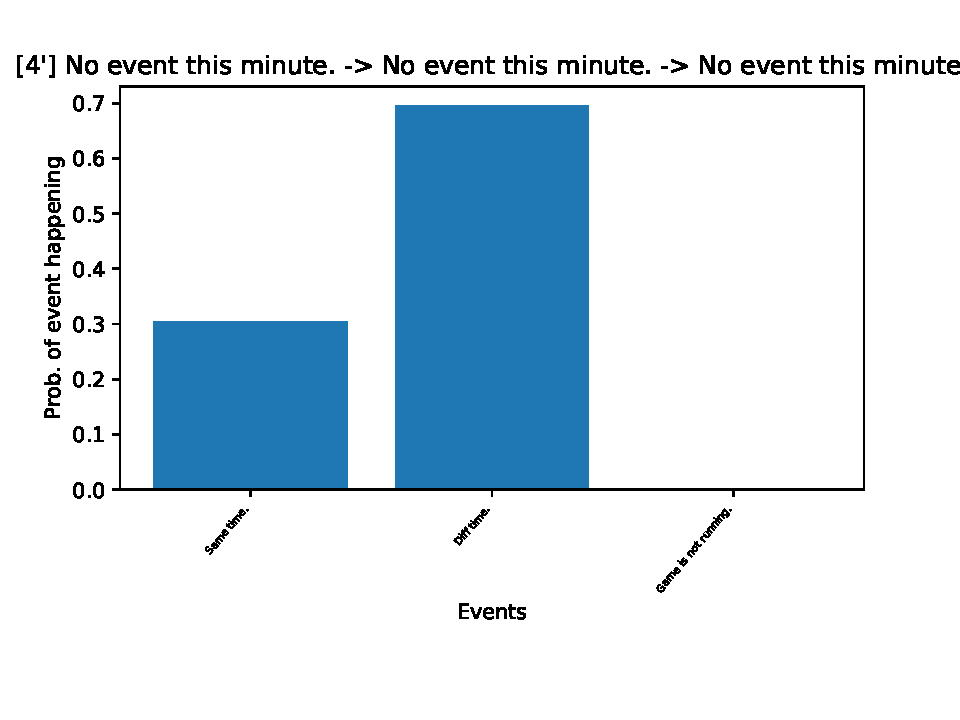
\includegraphics[width=125mm]{images/test_3}
\caption{Probabilities of all the different events after a goal by Real Madrid has been generated in the game between Real Madrid (home team) and Elche (away team). You can see the three previous events in the title of the graph.}
\label{fig:test_3}
\end{figure}

\begin{figure}[H]
\centering
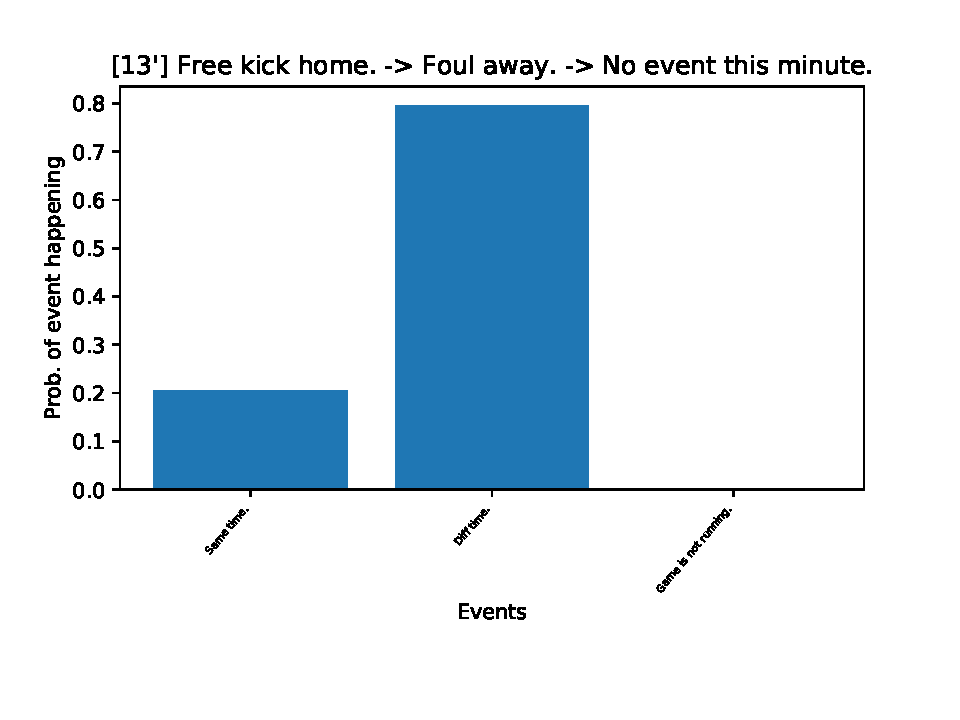
\includegraphics[width=125mm]{images/test_15}
\caption{Probabilities of all the different events during a very offensive action by Elche has been generated in the game between Real Madrid (home team) and Elche (away team). You can see the three previous events in the title of the graph.}
\label{fig:test_15}
\end{figure}

\begin{figure}[H]
\centering
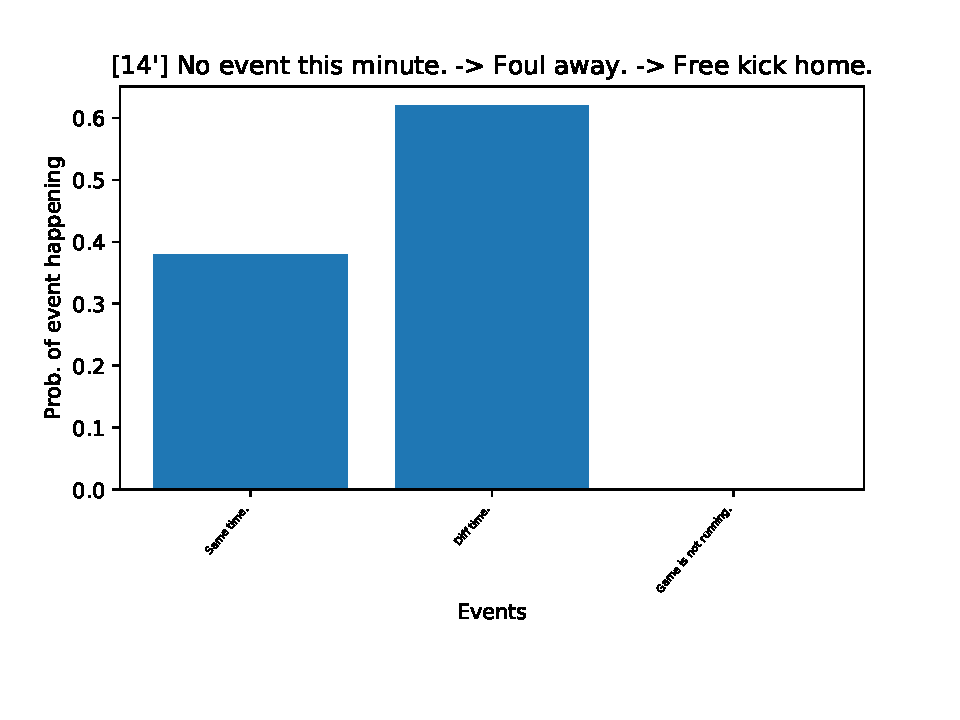
\includegraphics[width=125mm]{images/test_16}
\caption{Probabilities of all the different events after a goal by Real Madrid has been generated in the game between Real Madrid (home team) and Elche (away team). You can see the three previous events in the title of the graph.}
\label{fig:test_16}
\end{figure}

\begin{figure}[H]
\centering
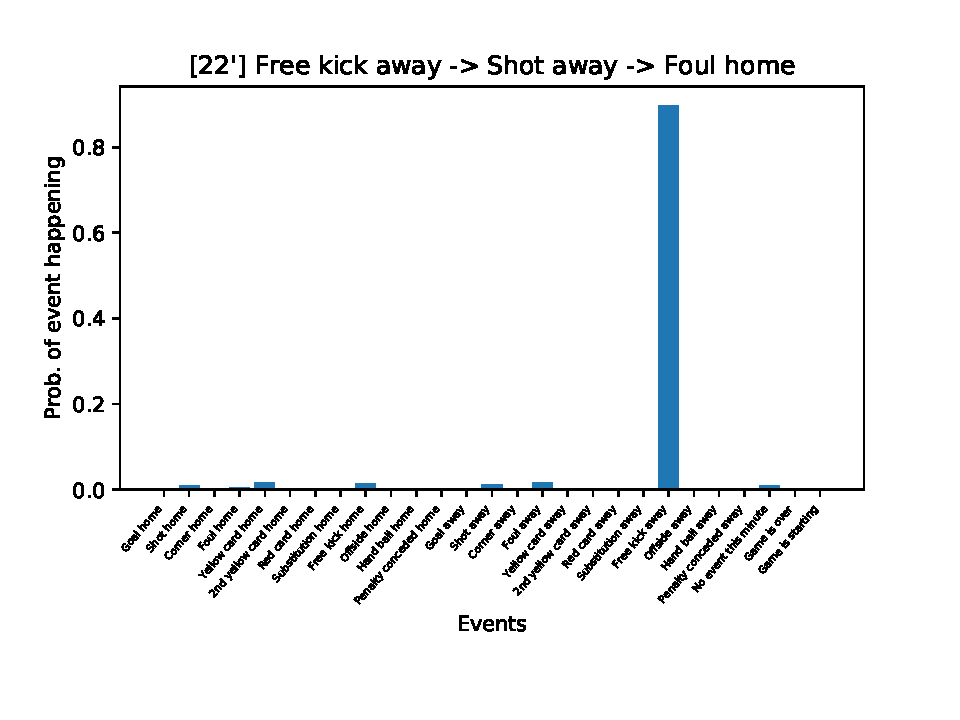
\includegraphics[width=125mm]{images/test_26}
\caption{Probabilities of all the different events after a foul committed by Real Madrid has been generated in the game between Real Madrid (home team) and Elche (away team). You can see the three previous events in the title of the graph.}
\label{fig:test_26}
\end{figure}

\begin{figure}[H]
\centering
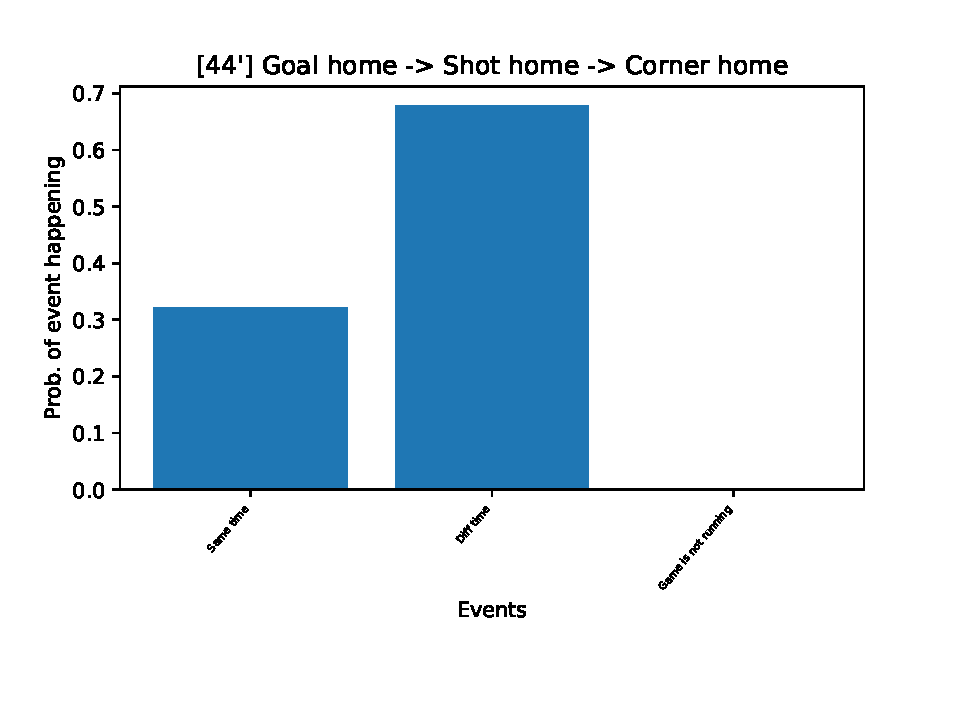
\includegraphics[width=125mm]{images/test_62}
\caption{Probabilities of all the different events during a very offensive action by Real Madrid has been generated in the game between Real Madrid (home team) and Elche (away team). You can see the three previous events in the title of the graph.}
\label{fig:test_62}
\end{figure}

We tried to generate a heatmap about transition probabilities of events, like the one shown in Section \ref{ssec:statistics}; Figure \ref{fig:same_side_event_influence_ours} and Figure \ref{fig:other_side_event_influence_ours} show transition probabilities for events for the same team, and other team respectively.

\begin{figure}[H]
\centering
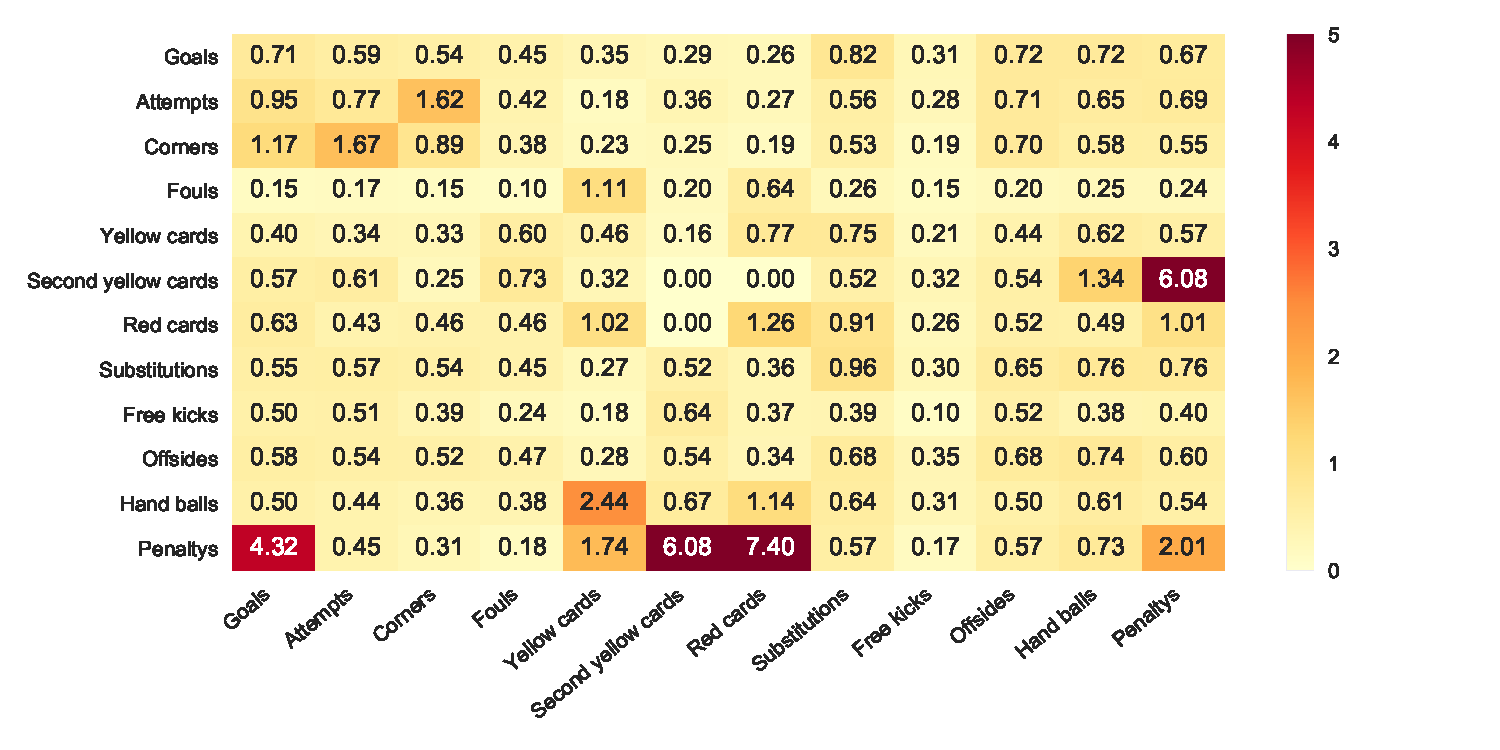
\includegraphics[width=125mm]{images/same_side_event_influence_ours}
\caption{Heatmap showing how each event has an influence on next events (for the same team) in our model.}
\label{fig:same_side_event_influence_ours}
\end{figure}

\begin{figure}[H]
\centering
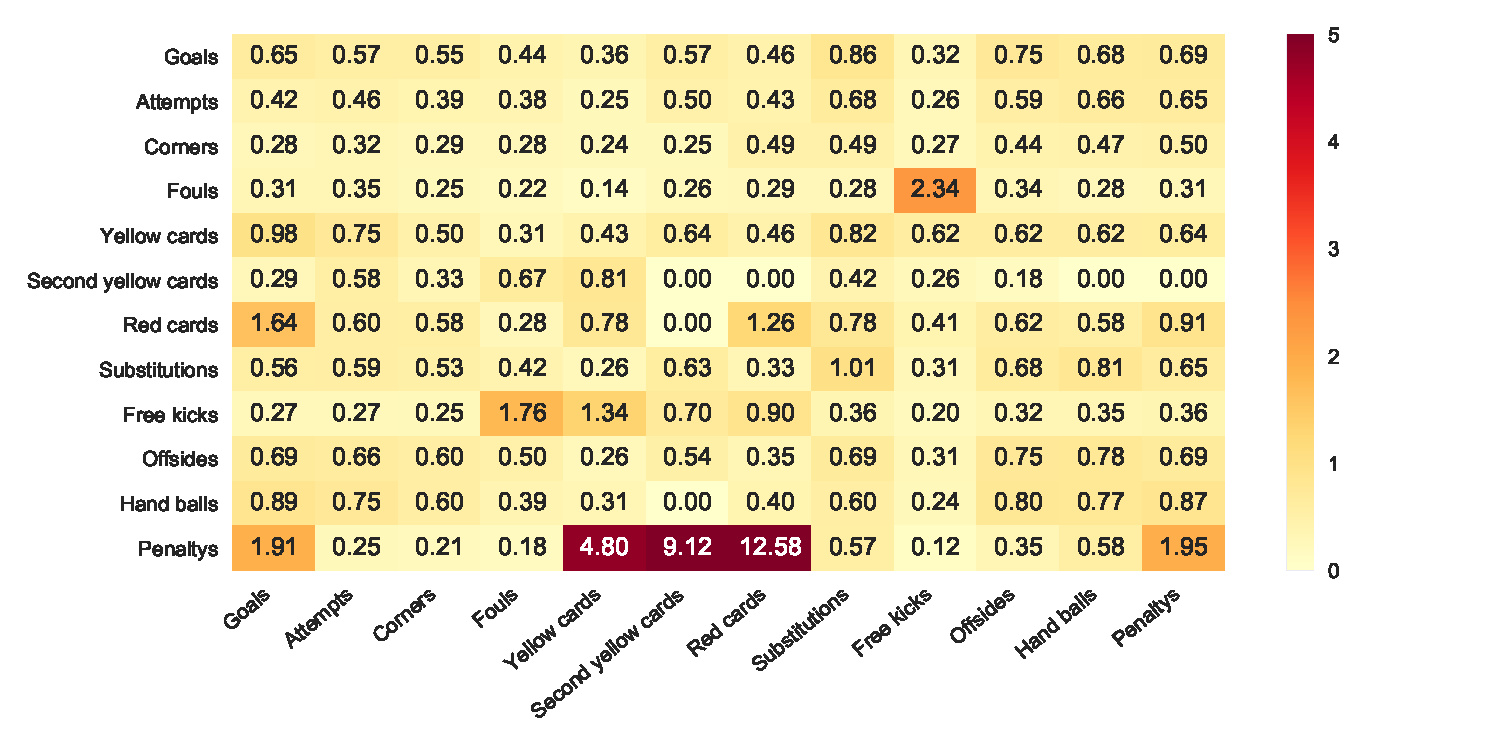
\includegraphics[width=125mm]{images/other_side_event_influence_ours}
\caption{Heatmap showing how each event has an influence on next events (for the other team) in our model.}
\label{fig:other_side_event_influence_ours}
\end{figure}

By looking and comparing with the heatmaps in Section \ref{ssec:statistics}, we can see a lot of similar things, which could convince us that our network has learned from those direct relations between events. We then tried to compute the ratio between the heatmaps for all the games and the heatmaps for the games we generated, to see if the numbers were somewhere around 1 for most pairs of events. Figure \ref{fig:ratio_same_side_event_influence} and Figure \ref{fig:ratio_other_side_event_influence} show those ratios for the heatmaps about events for the same team, and other team respectively.

\begin{figure}[H]
\centering
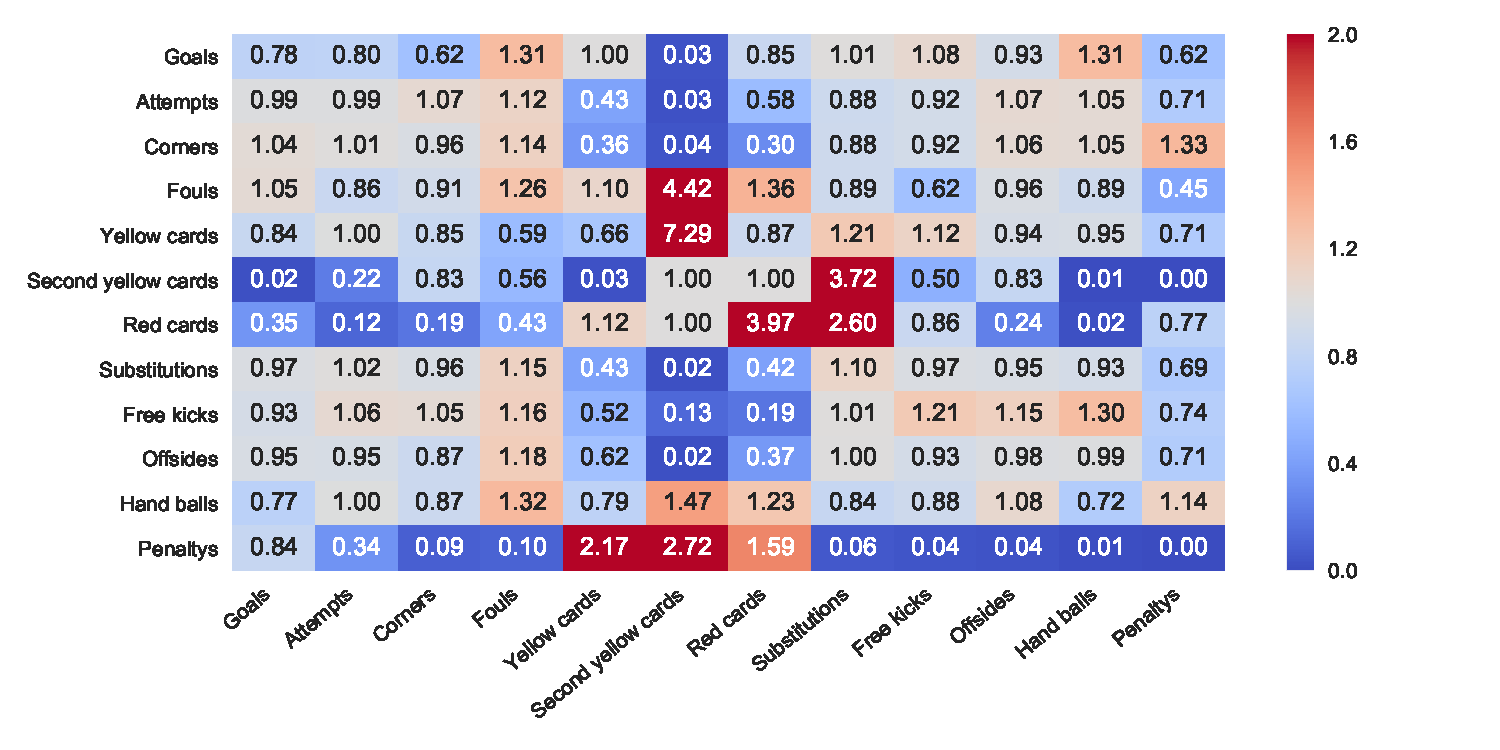
\includegraphics[width=125mm]{images/ratio_same_side_event_influence}
\caption{Heatmap showing the ratios between the influence of events on the next events (for the same team) for all the games and for the games generated by our model.}
\label{fig:ratio_same_side_event_influence}
\end{figure}

\begin{figure}[H]
\centering
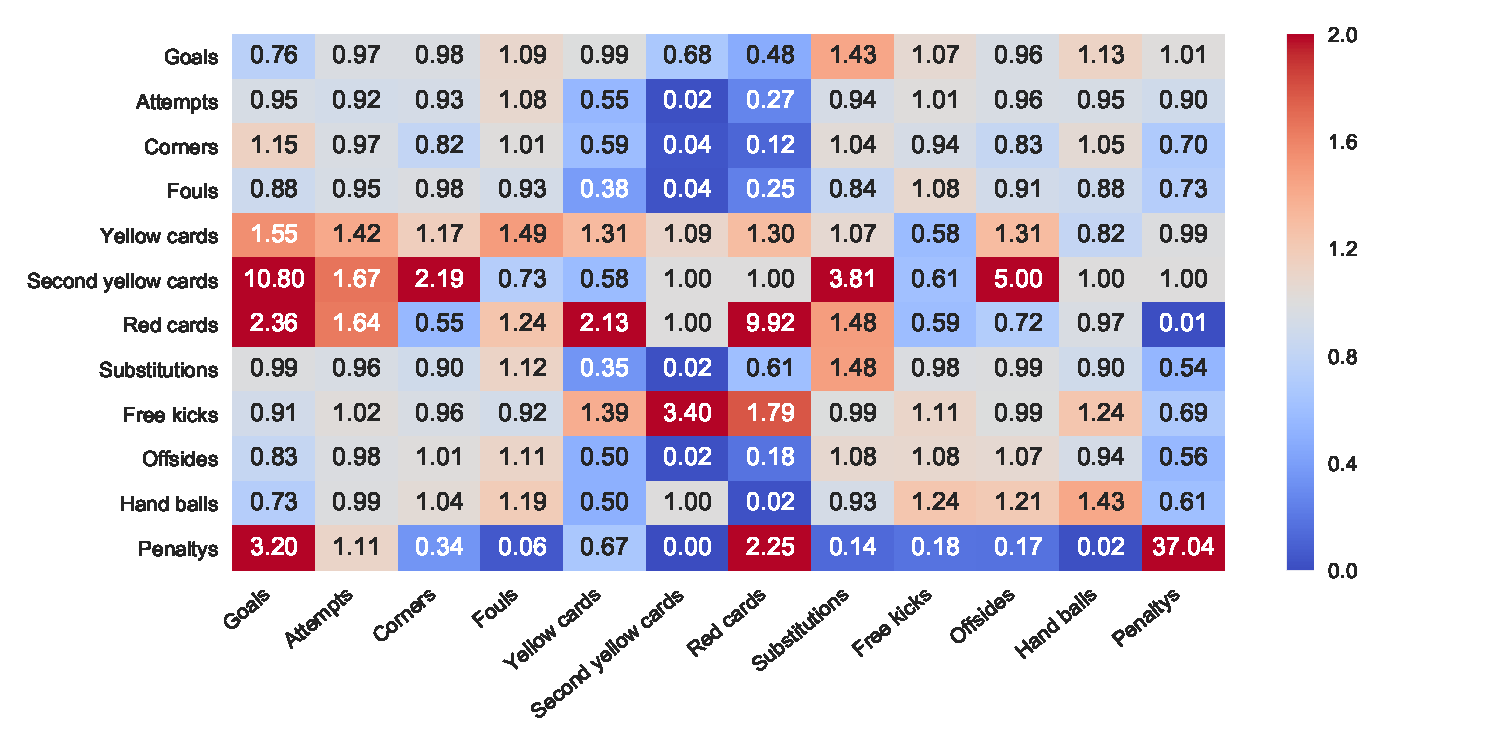
\includegraphics[width=125mm]{images/ratio_other_side_event_influence}
\caption{Heatmap showing the ratios between the influence of events on the next events (for the other team) for all the games and for the games generated by our model.}
\label{fig:ratio_other_side_event_influence}
\end{figure}

We see that we don't have the same influence on rare events, such as second yellow cards, red cards and penalties. This makes sense because there isn't enough occurrences of those events to followed or preceded by all the others to have reliable data that we can compare. If we remove those rows and columns, we see that most numbers are near 1, which shows that our model was able to correctly learn those relationships.

\end{appendices}

\end{document}

